% Generated by experiments/plot_ch3_empirical.py. Preamble: \usepackage{graphicx}
\begin{figure}[htbp]
  \centering
  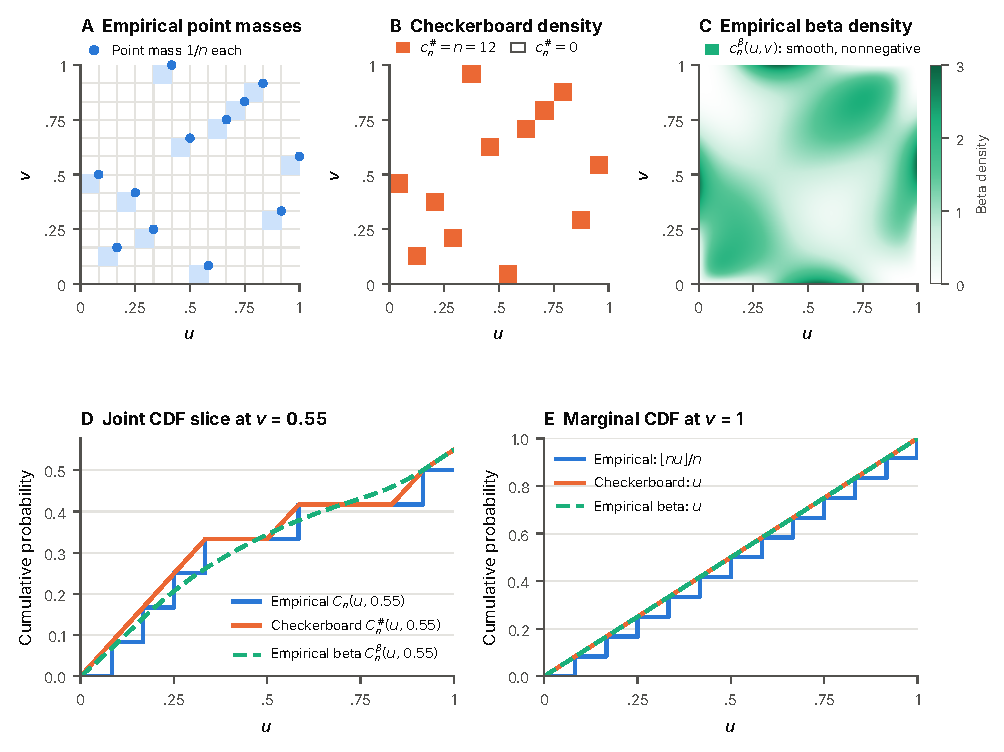
\includegraphics[width=\textwidth]{figures/fig_ch3_empirical}
  \caption{The empirical, empirical checkerboard and empirical beta copulas of one sample of
    $n = 12$ pairs drawn with latent Gaussian correlation $0.7$; all three use only the ranks.
    (A)~Scaled rank pairs $(R_i/n, S_i/n)$, each with mass $1/n$, at the upper-right corner of
    its grid cell. (B)~Checkerboard density: $n$ on each occupied cell and $0$ elsewhere.
    (C)~Beta density $c_n^{\beta}(u,v) = n^{-1}\sum_{i} f_{R_i}(u) f_{S_i}(v)$, with $f_r$ the
    $\mathrm{Beta}(r, n+1-r)$ density; the colour scale is truncated at $3$ (the maximum is
    $12$, at the corner of the pair ranked $(1,1)$). (D)~The three copulas at $v = 0.55$: the
    empirical copula is a step function; the checkerboard is piecewise linear and agrees with it
    at every grid vertex; the beta copula is smooth and does not interpolate those values.
    (E)~First margins ($v = 1$): $\lfloor nu \rfloor / n$ for the empirical copula, exactly $u$
    for the checkerboard and beta copulas (dashed curve overlays the solid one).}
  \label{fig:ch3-empirical}
\end{figure}
